The shared-memory parallelisation run was conducted on a machine called togian.
This system is a quad socket AMD Opteron 6366HE system giving it 64 cores paired
into 32 modules running at 1.8GHz. To provide consistent benchmarking results,
the turbo clock frequencies were disabled. The system has been fitted with 512GB
of DDR3 RAM. In terms of software, gfortran version 4.7.2 with MPICH 3.1.3 were
used for the majority of the evaluation. OpenMPI 1.8.4 performance was also
investigated.

\subsubsection{Default Mapping}

The first configuration under evaluation was the default setup for MPICH 3.1.3.
This default mapping assigns processes to cores in a round-robin fashion across
sockets. This spreads the runtime load between CPU sockets thus minimising the
load on the CPUs cache for small numbers of processes and maximises the chance
of achieving a higher turbo clock frequency if applicable.

\begin{figure}
    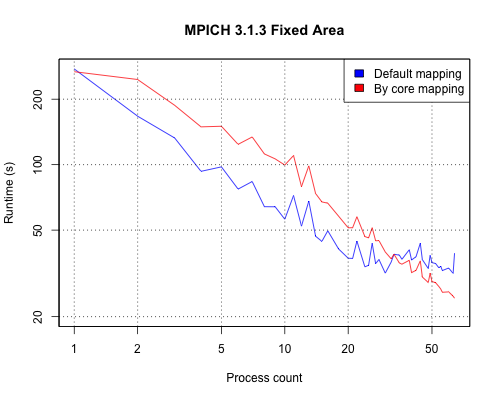
\includegraphics[width=0.5\textwidth]{graphs/MPICH313-fixed-area.png}
    \caption{MPICH 3.1.3 Fixed Area Runtimes}
    \label{fig:mpichfixedarea}
\end{figure}

Figure~\ref{fig:mpichfixedarea} shows linear improvements in runtime for a fixed
sized area. Single threaded performance has a runtime of 275.5 seconds with 64
threads completing its run in 39.2 seconds, a 7x improvement in computational
throughput.

The graph isn't as smooth as would normally be expected. This is as a direct
consequence to the mapping of processes over a two dimensional area. If the same
number of processes exist in both axes, then the performance is at its best
since the length of all halos are equal. If the process counts differ then they
cannot have a balanced layout since two halos will be significantly shorter than
the others. This difference acts as a bottleneck since the shorter halo
exchanges finish sooner then have to wait for the longer halo exchanges to
complete.

Figure~\ref{fig:mpichexpandingarea} shows good scaling of runtime where the
overall area under simulation grows at the same rate as the process count. A
single process executing on a 150x150x90 area takes 69.2 seconds to execute
whereas 64 processes executing on a 1200x1200x90 area takes 235.9 seconds to
execute. This equates to a 3.4x increase in runtime for a 64x increase in area,
improving throughput by 18.8x. Comparing this with the fixed area improvement of
7x, it is clear to see that to get the most benefit from the MPI parallelised
LES, it should be used to to calculate velocities over greater areas or at
greater resolutions than before. This is also as intuition would expect since
the setup cost of sending a message is fixed irrespective of the message size so
larger messages amortize the cost of the setup. Also, as the fixed area runs
gain processes, the ratio between time spent doing useful computation and
message sending decreases.

\begin{figure}
    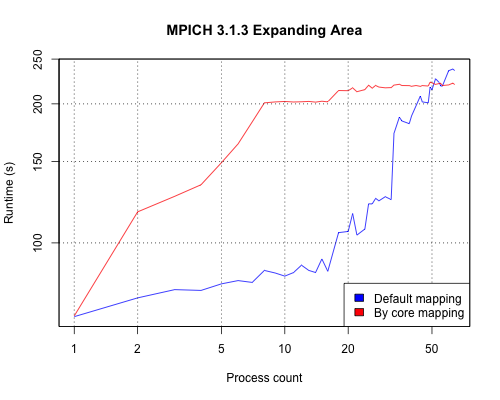
\includegraphics[width=0.5\textwidth]{graphs/MPICH313-expanding-area.png}
    \caption{MPICH 3.1.3 Expanding Area Runtimes}
    \label{fig:mpichexpandingarea}
\end{figure}

Towards the end of the graph there is a significant increase. This occurs on the
move from 32 to 33 processes. This is because at 32 processes, all sockets are
exactly `half full'. Each module has its own hardware thread active so each
process has its own floating point units. On the move to 33 processes, a process
will now have to share floating point units with another process. This will slow
down these processes and, by extension, the application overall. This is a
feature of the AMD CPU architecture and not something caused by MPI or the LES.

\subsubsection{By Core Mapping}

The second configuration under evaluation involved a minor change to MPICH
3.1.3. Instead of using the default mapping of processes to cores, mpiexec was
setup to assign processes to cores sequentially. This means a single socket will
be `filled up' with processes before moving on to the next. The rationale behind
this change was to increase the probability that a processes neighbours were on
the same socket. This is almost always now true for the left and right neighbour
which will be running on the previous and next core respectively. The primary
downsides are increased cache and floating point unit utilisation on smaller
process counts. For example, a four process run is now sharing the resources of
a single socket rather than each having the resources of their own socket.
Another downside is that the turbo frequency will be reduced quicker on
applicable systems since a socket will reach higher process counts sooner.

Figure~\ref{fig:mpichfixedarea} shows that, for the fixed area runs, the
performance difference is negligible. The lower process counts have poorer
performance however, once the 32 process boundary has been crossed, performance
is the same as the default mapping case.

Figure~\ref{fig:mpichexpandingarea} again shows good scaling of
runtime where the overall simulation area increases at the same rate as the
process count increases. It also shows more clearly that runtime levels out so
increases in area are `for free' when increasing the process count by the same
amount. Runtime now levels out at around 220 seconds which is a 7\% improvement
over the default mapping case. This change isn't massive but is consistent and
shows that tweaks outside of the code itself can benefit performance.

As expected, the performance at small process counts is significantly poorer
than in the default mapping case however since it is expected that an entire
shared-memory system or entire nodes would be dedicated to a single application
at any given time this degradation is deemed acceptable given the marginal
performance improvement at higher numbers of processes.

\subsubsection{MPICH versus OpenMPI}

There are two popular implementations of the MPI standard: MPICH and OpenMPI.
Other implementations include several derivatives of MPICH making MPICH one of
the most popular implementations available. OpenMPI is used in many of the
TOP500 supercomputers and is designed to act as an efficient implementation for
common case MPI use cases whereas MPICH acts as a high quality reference
implementation of the latest available MPI standard.

In addition to evaluating performance on MPICH version 3.1.3, the performance
characteristics of OpenMPI version 1.8.4 were also investigated. Many of the
configurations discussed for MPICH were repeated for OpenMPI to enable direct
comparisons between runtimes.

There is no tangible performance difference between MPICH 3.1.3 and OpenMPI
1.8.4. MPICH 3.1.3 is moderately faster but OpenMPI is less than 10\% slower for
high process counts. It can be concluded that use of either MPI implementation
will yield similar speedups as each other. With many other MPI implementations
being based on MPICH, the same performance characteristics could be expected
from those as well.
